\documentclass[article]{BJTU-thesis}
\usepackage{url}
\usepackage{booktabs}
\setcounter{tocdepth}{4}
\setcounter{secnumdepth}{4}
\hypersetup{hidelinks}
\renewcommand\thesection{\arabic {section}}
\renewcommand\thefigure{\arabic {figure}}
\definecolor{mygreen}{rgb}{0.15,0.66,0.7}
\definecolor{myblue}{rgb}{0,0,164}
\definecolor{mygray}{rgb}{0.6,0.65,0.74}
\definecolor{mymauve}{rgb}{0.58,0,0.82}
\lstset{
	numbers=left, 
	breaklines=true,              
	columns=fixed, 
	commentstyle=\color{mygray}\rmfamily\itshape,    
	keywordstyle=\color{myblue},    
	stringstyle=\color{mygreen}\ttfamily,  
	rulesepcolor=\color{red!20!green!20!blue!20} }

%%%%%%%%%%%%%%%填写封面信息%%%%%%%%%%%%%%%%%%%%
\authora{汤新宇  17301137}
\authorb{陈嘉琪  17301060}
\authorc{刘歆怡  17301129}
\authord{唐{\color{white}哈}麒  17301138}
\authorf{张钰铎  17301145}
\comment{同{\color{white}哈}等{\color{white}哈}贡{\color{white}哈}献}
%\studentNumber{16121248}
\advisor{冀振燕}
%\advisorTitle{教授}
%\degreeType{学术型}
%\major{机械制造}
%\researchArea{切削力分析}
\title{OWL 入侵监测系统设计}
\bibliographystyle{unsrt} % BibTex
%\englishtitle{The Path Planning of Blade Machining Tool Based on Cutting Force Analysis.}
%%%%%%%%%%%%%%%%%%%%%%%%%%%%%%%%%%%%%%%%%%%%%%
%\setmainfont{Times New Roman}
\bibliographystyle{unsrt} % BibTex
\begin{document}
	\makecover
	
	\tableofcontents
	\newpage

	\newpage
	\setcounter{page}{1}
	\section{系统简介}
	近年来,随着计算机视觉和网络技术的发展,互联网+安防的应用场景逐渐走进了大众的视野。例如基于实时的视频流,利用图像识别功能,自动检测视频中的运动物体,通过包括后端数据处理和前端 web 页面实时显示结果的系统,被广泛应用在小区入侵监测、智能家居的安防和老人智能看护等领域。在此基础上,加入人脸识别系统,结合其他的智能产品,即可实现高度自动化的物联网自动化运行环境。此外,借助云计算技术,将异常图像上传至云服务器,配合手机APP,可实达到全方位、实时监控的目的。
	
	本项目拟借助 Raspberry Pi 和 Pi camera 模拟应用场景中的监控设备,在监控端、服务器和前端网页之间通过 WebSocket 进行数据传输,实现仓库管理场景下的实时监控、入侵监测等功能。系统概貌如\textbf{图\ref{fig:fig1}}所示,开发环境如\textbf{表\ref{tab:tab1}}所示。
	
	\begin{figure}[!htb]
		\centering
		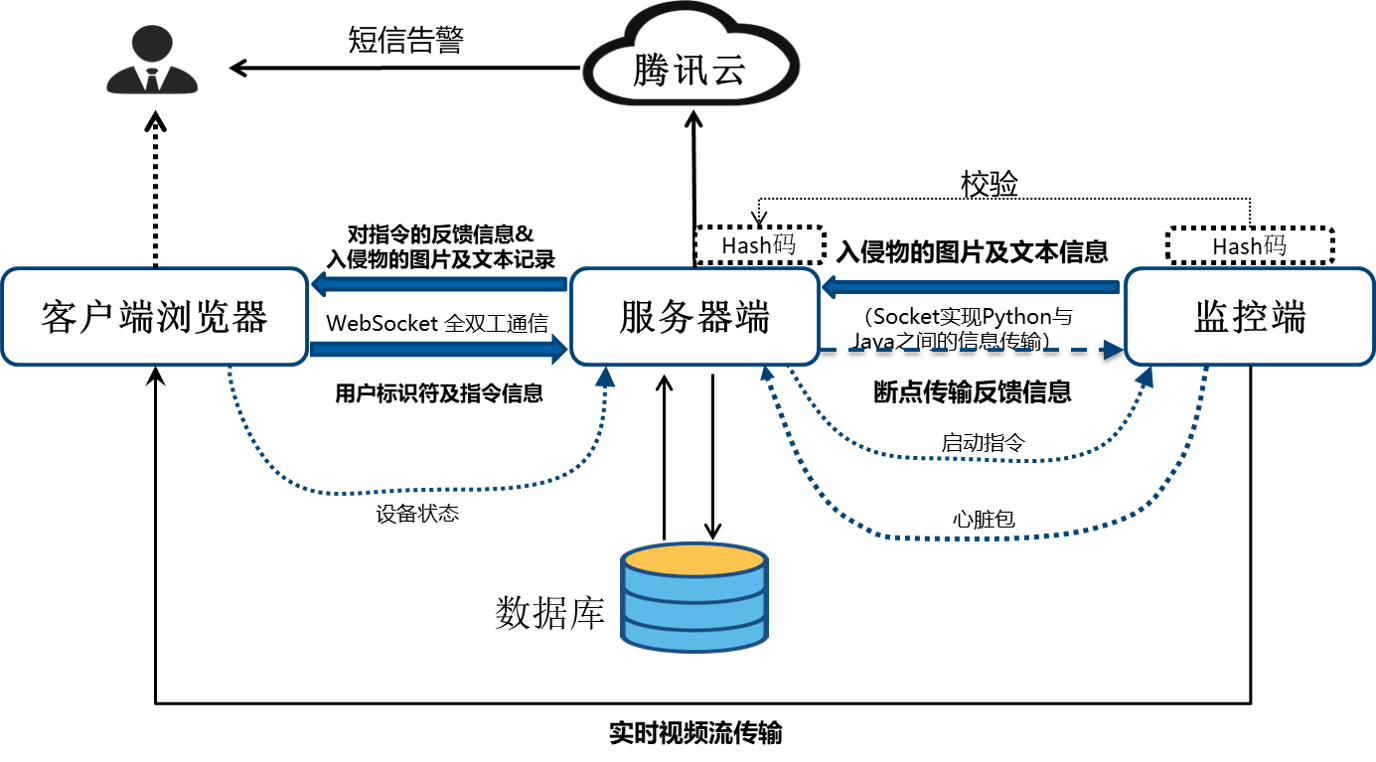
\includegraphics[scale=0.6]{img/1.png}
		\caption{系统概貌图}\label{fig:fig1}
	\end{figure}

	\begin{table}[!htbp]
		\centering
		\caption{开发环境表}
		\label{tab:tab1}
		\begin{tabular}{|c|c|c|}
			\hline
			& 名称 & 版本 \\ \hline
			操作系统 & Windows 10 & Windows SDK 10.0.17763.0 \\ \hline
			数据库 & MySQL & 8.0.16 \\ \hline
			监控端 & Python & 3.5 \\ \hline
			服务器端 & Java & JDK 8 \\ \hline
			客户端 & Vue、Nuxt.js &  \\ \hline
		\end{tabular}
	\end{table}
	
	
\section{功能描述}
\subsection{监控端}
\begin{figure}[!htbp]
	\centering
	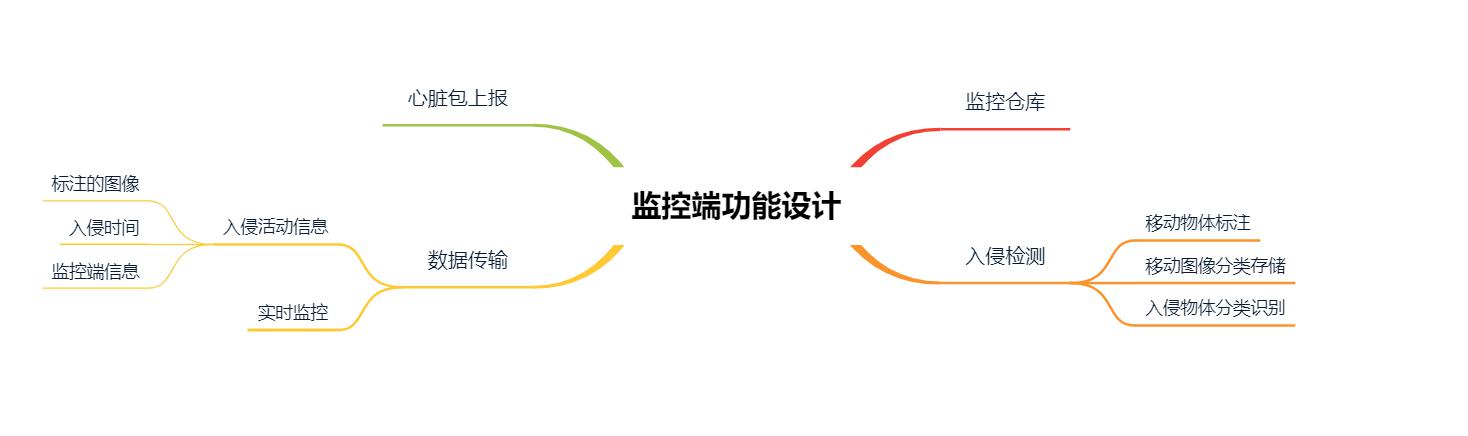
\includegraphics{img/2.jpg}
	\caption{监控端功能示意图}\label{fig:fig2}
\end{figure}

如\textbf{图\ref{fig:fig2}}所示,监控端的主要功能需求为
\begin{enumerate}
	\item 在完成监控端设备的安装和配置后,监控端通过外置镜头对仓库
	进行基本监控功能;
	\item 通过 Background subtraction 方法对视野范围内的画面进行移动物体监测,对移动物体进行标注和分类存储;
	\item 将监测到的入侵活动,以包含设备序列号、时间、入侵物体分类和异常图片及其哈希值等的数据包向服务器传输;
	\item 对实时监控视频流进行编码并传输;
	\item 传输心脏包。
\end{enumerate}

\subsection{服务器}
\begin{figure}[!htbp]
	\centering
	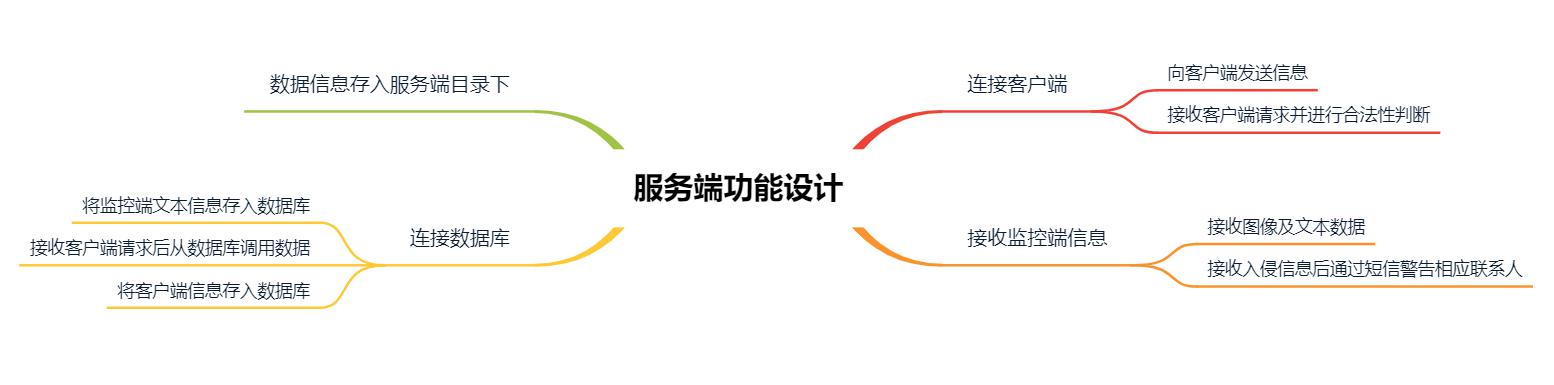
\includegraphics{img/3.jpg}
	\caption{服务器功能示意图}\label{fig:fig3}
\end{figure}
如\textbf{图\ref{fig:fig3}}所示,服务器的主要功能需求为
\newpage
\begin{enumerate}
	\item 持续监听来自监控端的连接请求,接收来自监控端的数据(支持断点续传);
	\item 将图片、文本信息信息存储至数据库;
	\item 通过短信、推送等方式告警客户联系人;
	\item 依据客户端指令调取数据库信息并反馈。
	
\end{enumerate}
\subsection{客户端}
\begin{figure}[!htbp]
	\centering
	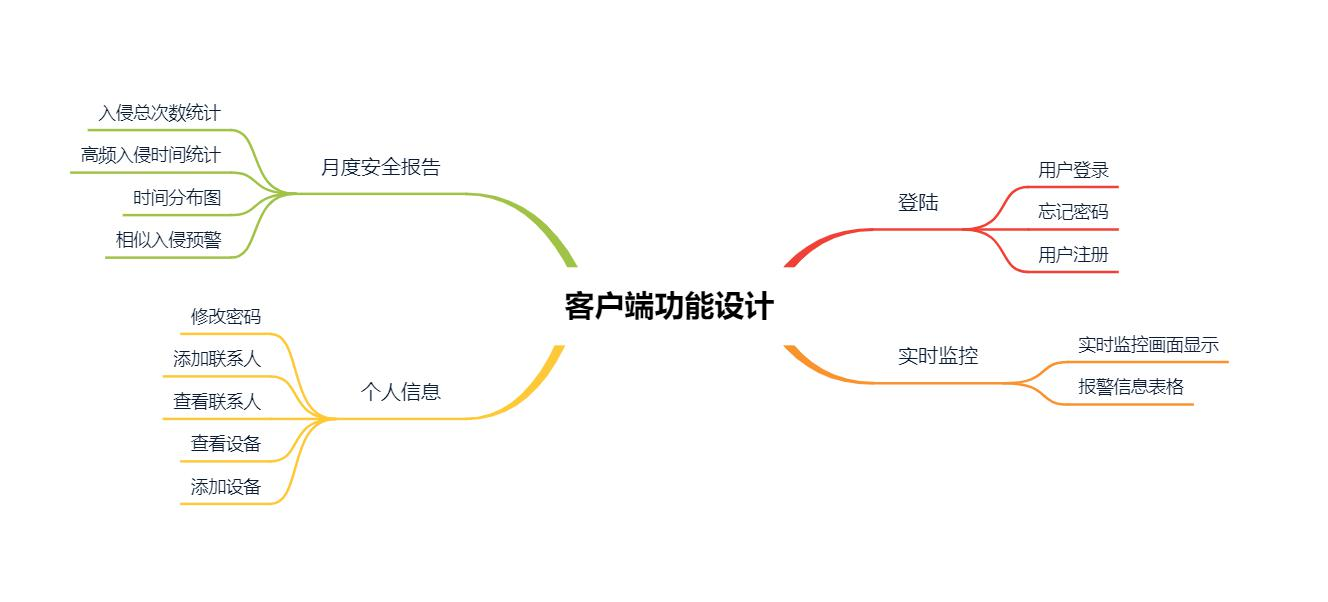
\includegraphics{img/4.jpg}
	\caption{客户端功能示意图}\label{fig:fig4}
\end{figure}
如\textbf{图\ref{fig:fig4}}所示,客户端的主要功能需求为
\newpage
\begin{enumerate}
	\item 用户注册/登录,核实监控端设备序列号;
	\item 修改个人信息,包括但不限于修改密码、添加联系人等;
	\item 查看实时监控画面、报警信息和月度安全报告;
	\item 设置安全时段。
	
\end{enumerate}

\section{系统设计}
\subsection{面向对象的设计原则}

根据上一节的功能描述,监控端和服务器的简化类图如\textbf{\ref{fig:fig25}}所示:

\begin{figure}[!htbp]
	\centering
	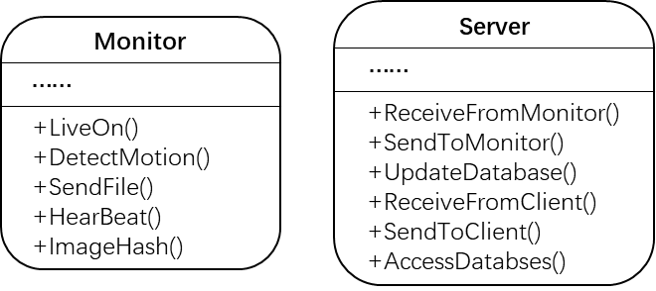
\includegraphics[scale=1]{img/22.png}
	\caption{监控端和服务器类图}\label{fig:fig25}
\end{figure}
\subsubsection{单一职责原则(SRP)}

\textbf{概念} 指一个类或者模块应该有且只有一个改变的原因。

\textbf{案例1}  原项目监控端拥有三个线程,分别是传输实时视频流(LiveOn),心跳包(HeartBeat)和发送对移动物体分析后的数据(DetectMotion、SendFile)。而这三项功能都在一个大的模块中工作,每一个功能的改变都会使其发生改变,因而违反单一职责原则。

\textbf{案例2} 服务器负责的工作是在监控端、数据库以及前端之间的数据传输。而对每一项功能并没有进行完美的分离,冗余在了同一块模块中,对于某一模块,修改时一定会有多种原因,这违背了单一职责原则。

\subsubsection{开放封闭原则(OCP)}
\textbf{概念} 软件实体应该是可扩展,而不可修改的。也就是说,对扩展是开放的,而对修改是封闭的。

\textbf{案例} 对于服务器和前端数据传输,通过设计和编码,在传输的数据包中包含标识特定功能的独立编码,服务器对接收到的数据包进行解析,通过判断功能编码,从数据库中获得相应数据并传回前端进行渲染。如果前端添加新的功能,对于原项目的服务器,由于对每个模块的设计并不到位,所以其在添加新功能时的修改方式一定会采用修改代码添加判断分支的方式,而不是使用扩展的方式,所以这一部分是违反开放封闭原则的。

\subsubsection{里氏替换原则(LSP)}
\textbf{概念} 程序中的对象应该是可以在不改变程序正确性的前提下被它的子类所替换的。

\textbf{案例} 原项目中鲜有继承关系,故没有涉及到里式替换原则。

\subsubsection{依赖倒置原则(DIP)}
\textbf{概念} 程序要依赖于抽象接口,不要依赖于具体实现。简单的说就是要求对抽象进行编程,不要对实现进行编程,这样就降低了客户与实现模块间的耦合。

\textbf{案例} 原项目中,服务器对数据库的访问是在判断前端传输的数据包中的唯一功能编码进入到不同的分支,在不同的分支结构中,通过 JDBC 和 SQL 语句从数据库中获得所需的数据,因而业务逻辑和数据访问依赖于数据层的具体实现,违反了依赖倒置原则。\newline

\textbf{修改方案综述}

\begin{figure}[!htbp]
	\centering
	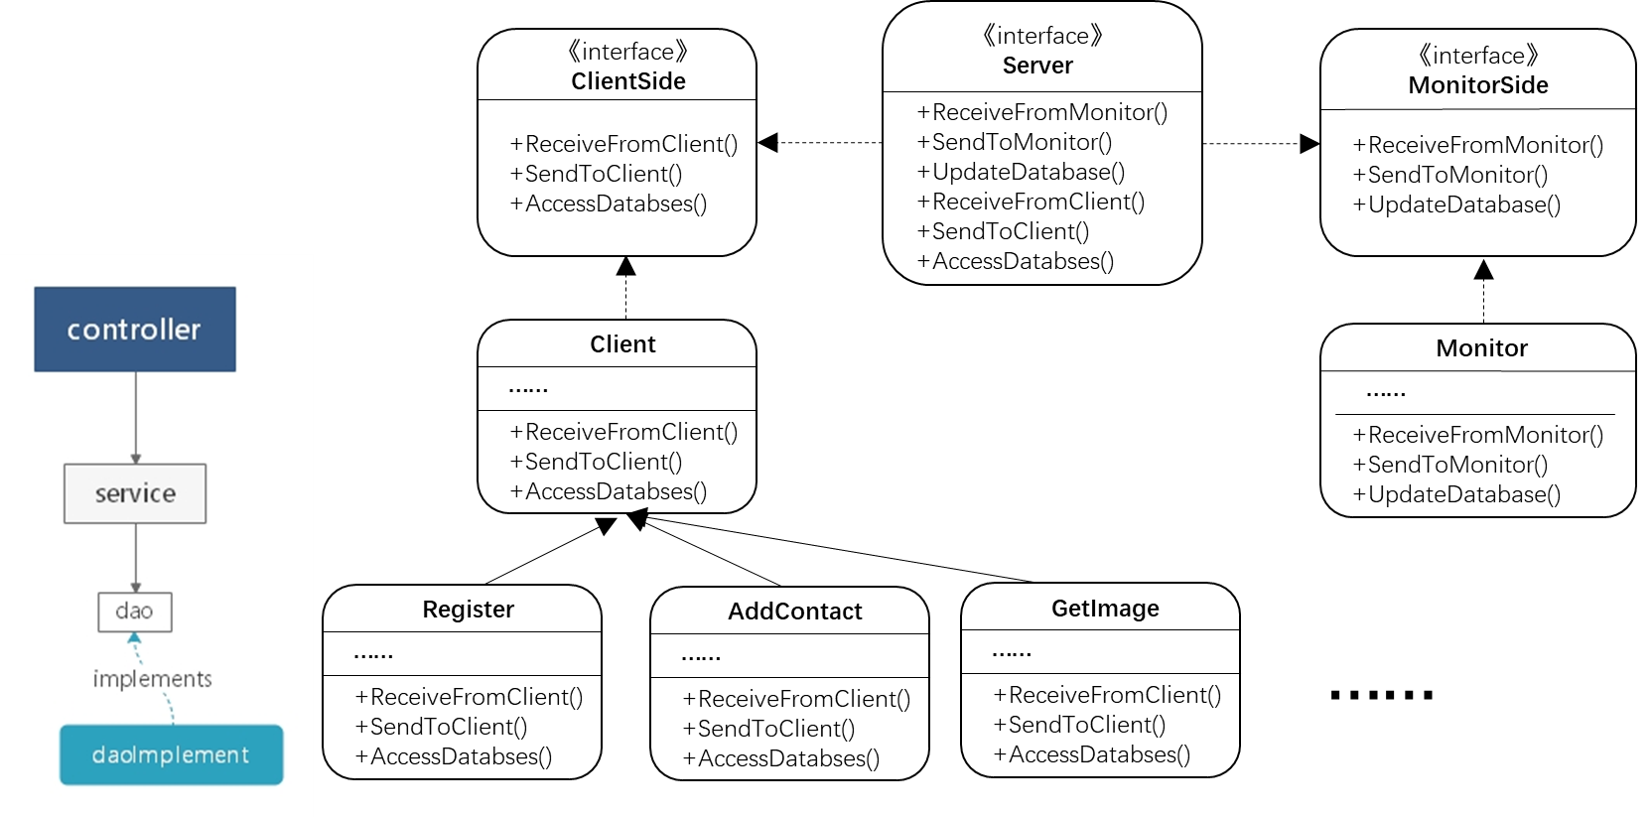
\includegraphics[scale=0.6]{img/23.png}
	\caption{服务器类图(修改后)}\label{fig:fig26}
\end{figure}

以服务器设计为例,对违反上述原则的设计进行修改,其简化的类图如\textbf{\ref{fig:fig26}}所示。

将服务器设计为包含可以与监控端、前端进行数据传输和访问数据库的“胖接口”(Server),将该接口分为与监控端交互(MonitorSide)和与客户端交互(ClientSide)的接口,将服务器的两个职责分离,满足了单一职责原则和接口分离原则,通过 Client 类和 Monitor 类实现这两个接口,作为与客户端和监控端交互的父类。以客户端为例,对于不同的功能,如注册/登录、添加联系人、查看异常图片,可通过继承的方式复写父类方法,在不同的子类中调用不同的方法,实现特定功能,这样一来,增加新的功能不必修改源代码,而是以继承或插件的形式实现,满足了开放封闭原则。对于每一个子类,都可以替代其基类型,满足了里式替换原则。此外,将数据访问层和数据层以 spring boot 的分层模式,将原本不合理的依赖关系进行修正,满足了依赖倒置原则。

\subsubsection{接口分离原则(ISP)}

\textbf{概念} 客户程序不应该被迫依赖其不使用的方法。将胖接口分解成多个接口,每个接口服务特定类型的客户程序。

\textbf{案例} 客户程序不应该被迫依赖其不使用的方法,在项目修改过程中,我们消除了多职责的类,将胖接口分解成多个接口,每个接口服务特定的客户程序。

\textbf{案例一:正确案例}
在后端服务器的代码部分,数据传输类WebSocketTest中调用了Constants接口。Constants接口中定义了注册、登录、修改密码时返回的编码或错误码,代码结构如\textbf{图\ref{fig:fig11}}:

\begin{figure}[!htbp]
	\centering
	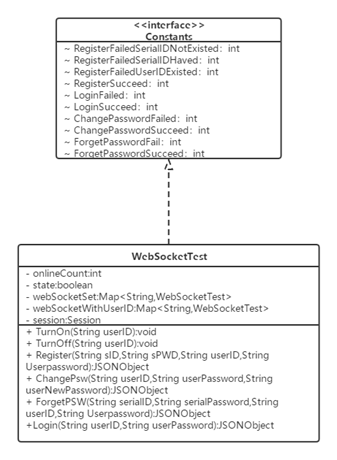
\includegraphics[scale=0.8]{img/11.png}
	\caption{服务器部分代码结构图}\label{fig:fig11}
\end{figure}

在用户注册时,Register函数中调用接口:

\lstinputlisting[language=Java,firstline=1,lastline=2]{code/2.java}

在用户修改密码时,ChangePsw函数中调用接口:

\lstinputlisting[language=Java,firstline=4,lastline=5]{code/2.java}

\newpage
在用户忘记密码时,ForgetPsw函数中调用接口:

\lstinputlisting[language=Java,firstline=7,lastline=8]{code/2.java}

在用户登录时,Login函数中调用接口:

\lstinputlisting[language=Java,firstline=10,lastline=11]{code/2.java}

客户程序功能包括登录、注册、修改密码、忘记密码等,内聚在一个类之中,调用Constants接口,没有被迫依赖接口中不使用的方法。接口中也没有定义冗余的常量,仅负责定义登陆注册相关的返回码,职责单一,服务特定类型的客户程序。

\textbf{案例二:修正案例} 前端包的初始设计如\textbf{图\ref{fig:fig12}}:

\begin{figure}[!htbp]
	\centering
	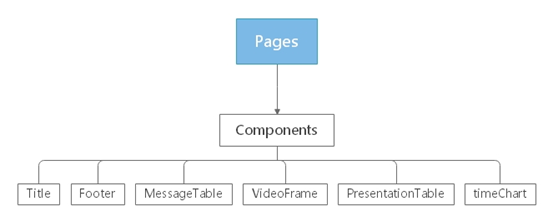
\includegraphics[scale=0.8]{img/8.png}
	\caption{前端包设计图}\label{fig:fig12}
\end{figure}

\newpage
在前端包的设计中,初始设计没有引入接口设计,直接定义组件类的项目结构不符合稳定抽象原则,导致前端的组件不好扩展。在此基础上我们进行了初步的接口设计,如\textbf{图\ref{fig:fig13}}所示:

\begin{figure}[!htbp]
	\centering
	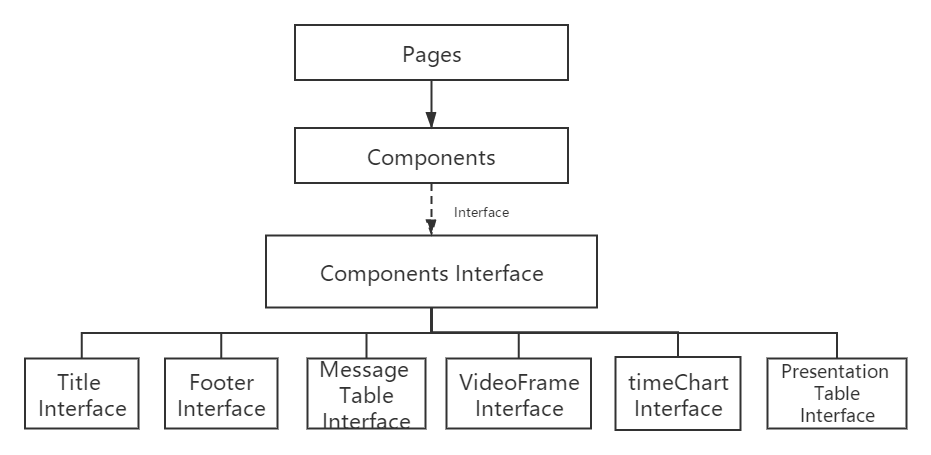
\includegraphics[scale=0.4]{img/13.png}
	\caption{前端包设计图(修改后)}\label{fig:fig13}
\end{figure}

一个Components Interface 中耦合了太多组件功能,导致接口较胖,在重用的过程中,存在客户程序被迫依赖其不使用的方法的情况。故我们在此基础上消除了多职责的接口,将胖接口分解成多个接口,每个接口服务特定的客户程序。根据接口分离原则,我们又对前端包的接口设计进行了如\textbf{图\ref{fig:fig14}}的修改:

\begin{figure}[!htbp]
	\centering
	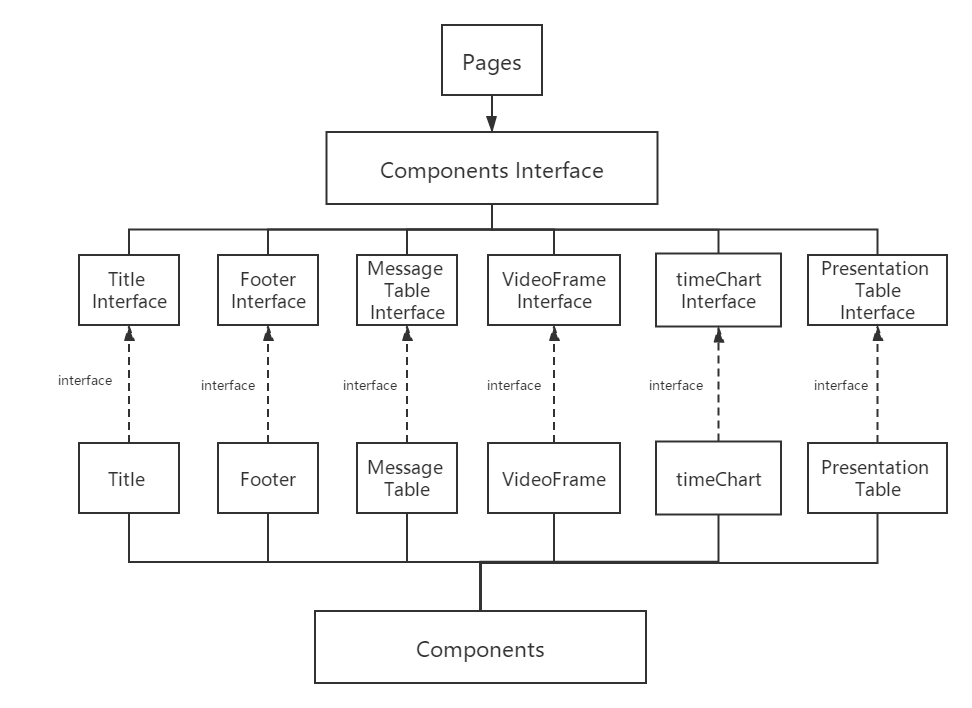
\includegraphics[scale=0.4]{img/12.png}
	\caption{前端包设计图}\label{fig:fig14}
\end{figure}

\newpage

修改后的结构满足了接口分离原则,但不具有高内聚性,最终我们根据包的内聚性相关原则,设计的前端包结构如\textbf{图\ref{fig:fig15}}:

\begin{figure}[!htbp]
	\centering
	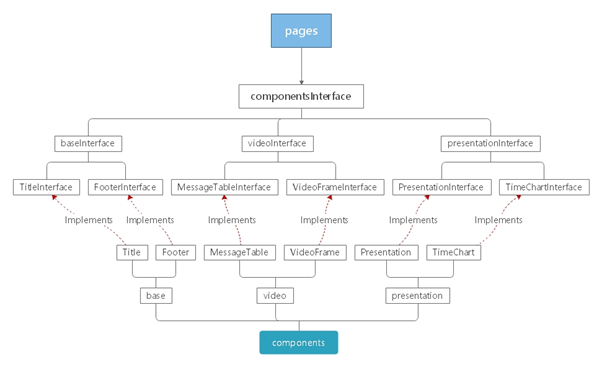
\includegraphics[scale=0.7]{img/14.png}
	\caption{前端包设计图}\label{fig:fig15}
\end{figure}

\subsection{包的设计原则}

\subsubsection{重用发布等价原则(REP)}
\textbf{概念} 重用的粒度与发布的粒度等价,一起重用的类一起发布。

\textbf{重用:}可以重用的代码是指利用这些代码的系统不需要看具体的代码,只要适当的时机替换掉静态的库就能够正常工作。

\textbf{发布:}包是相关的类的集合,换言之一个类基本上都和其他的一些有依赖关系。因此 、发布的最小单位一般认为是一个包。

\textbf{案例} 重用发布等价原则(REP)要求重用的粒度与发布的粒度等价。这就要求每次发布的包具有高内聚低耦合的特点,具有可重用性。
经过修改后,项目后端服务器的结构如\textbf{图\ref{fig:fig10}}所示:

\begin{figure}[!htbp]
	\centering
	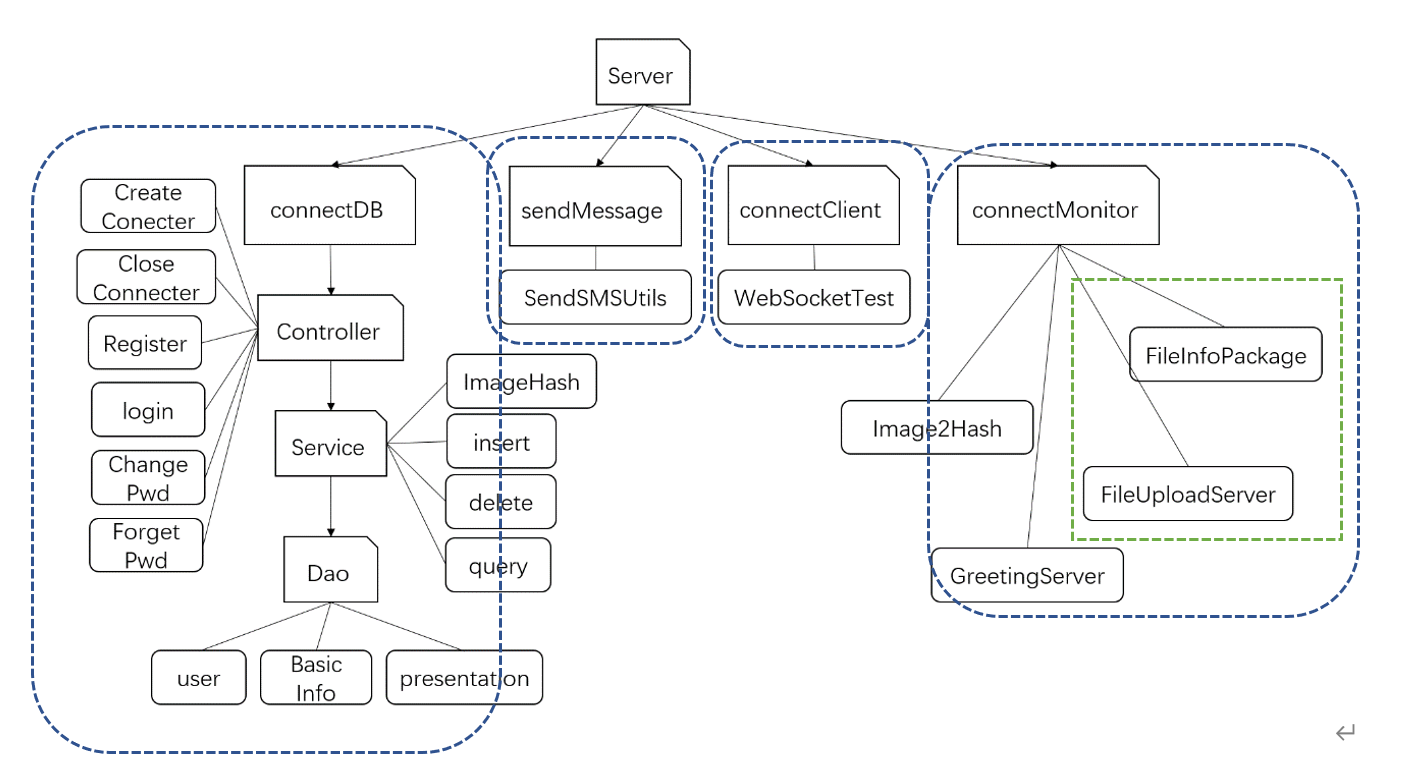
\includegraphics[scale=0.6]{img/10.png}
	\caption{客户端组件结构图(修改后)}\label{fig:fig10}
\end{figure}

在分包的过程中,我们把可复用的类放到一组包中,把不可复用的类放到另一组包中。每次发布时,按功能发布包,每个包的内容是为了同一个重用的目的编写的,每个包均是高内聚的,包内的类相互依赖。

\subsubsection{共同重用原则(CRP)}
\textbf{概念} 包中的类一起重用。如果你重用包中的一个类,则要重用包中所有的类。


\textbf{案例1:正确案例} 后端服务器的整体代码结构如\textbf{图\ref{fig:fig5}}所示:

\begin{figure}[!htbp]
	\centering
	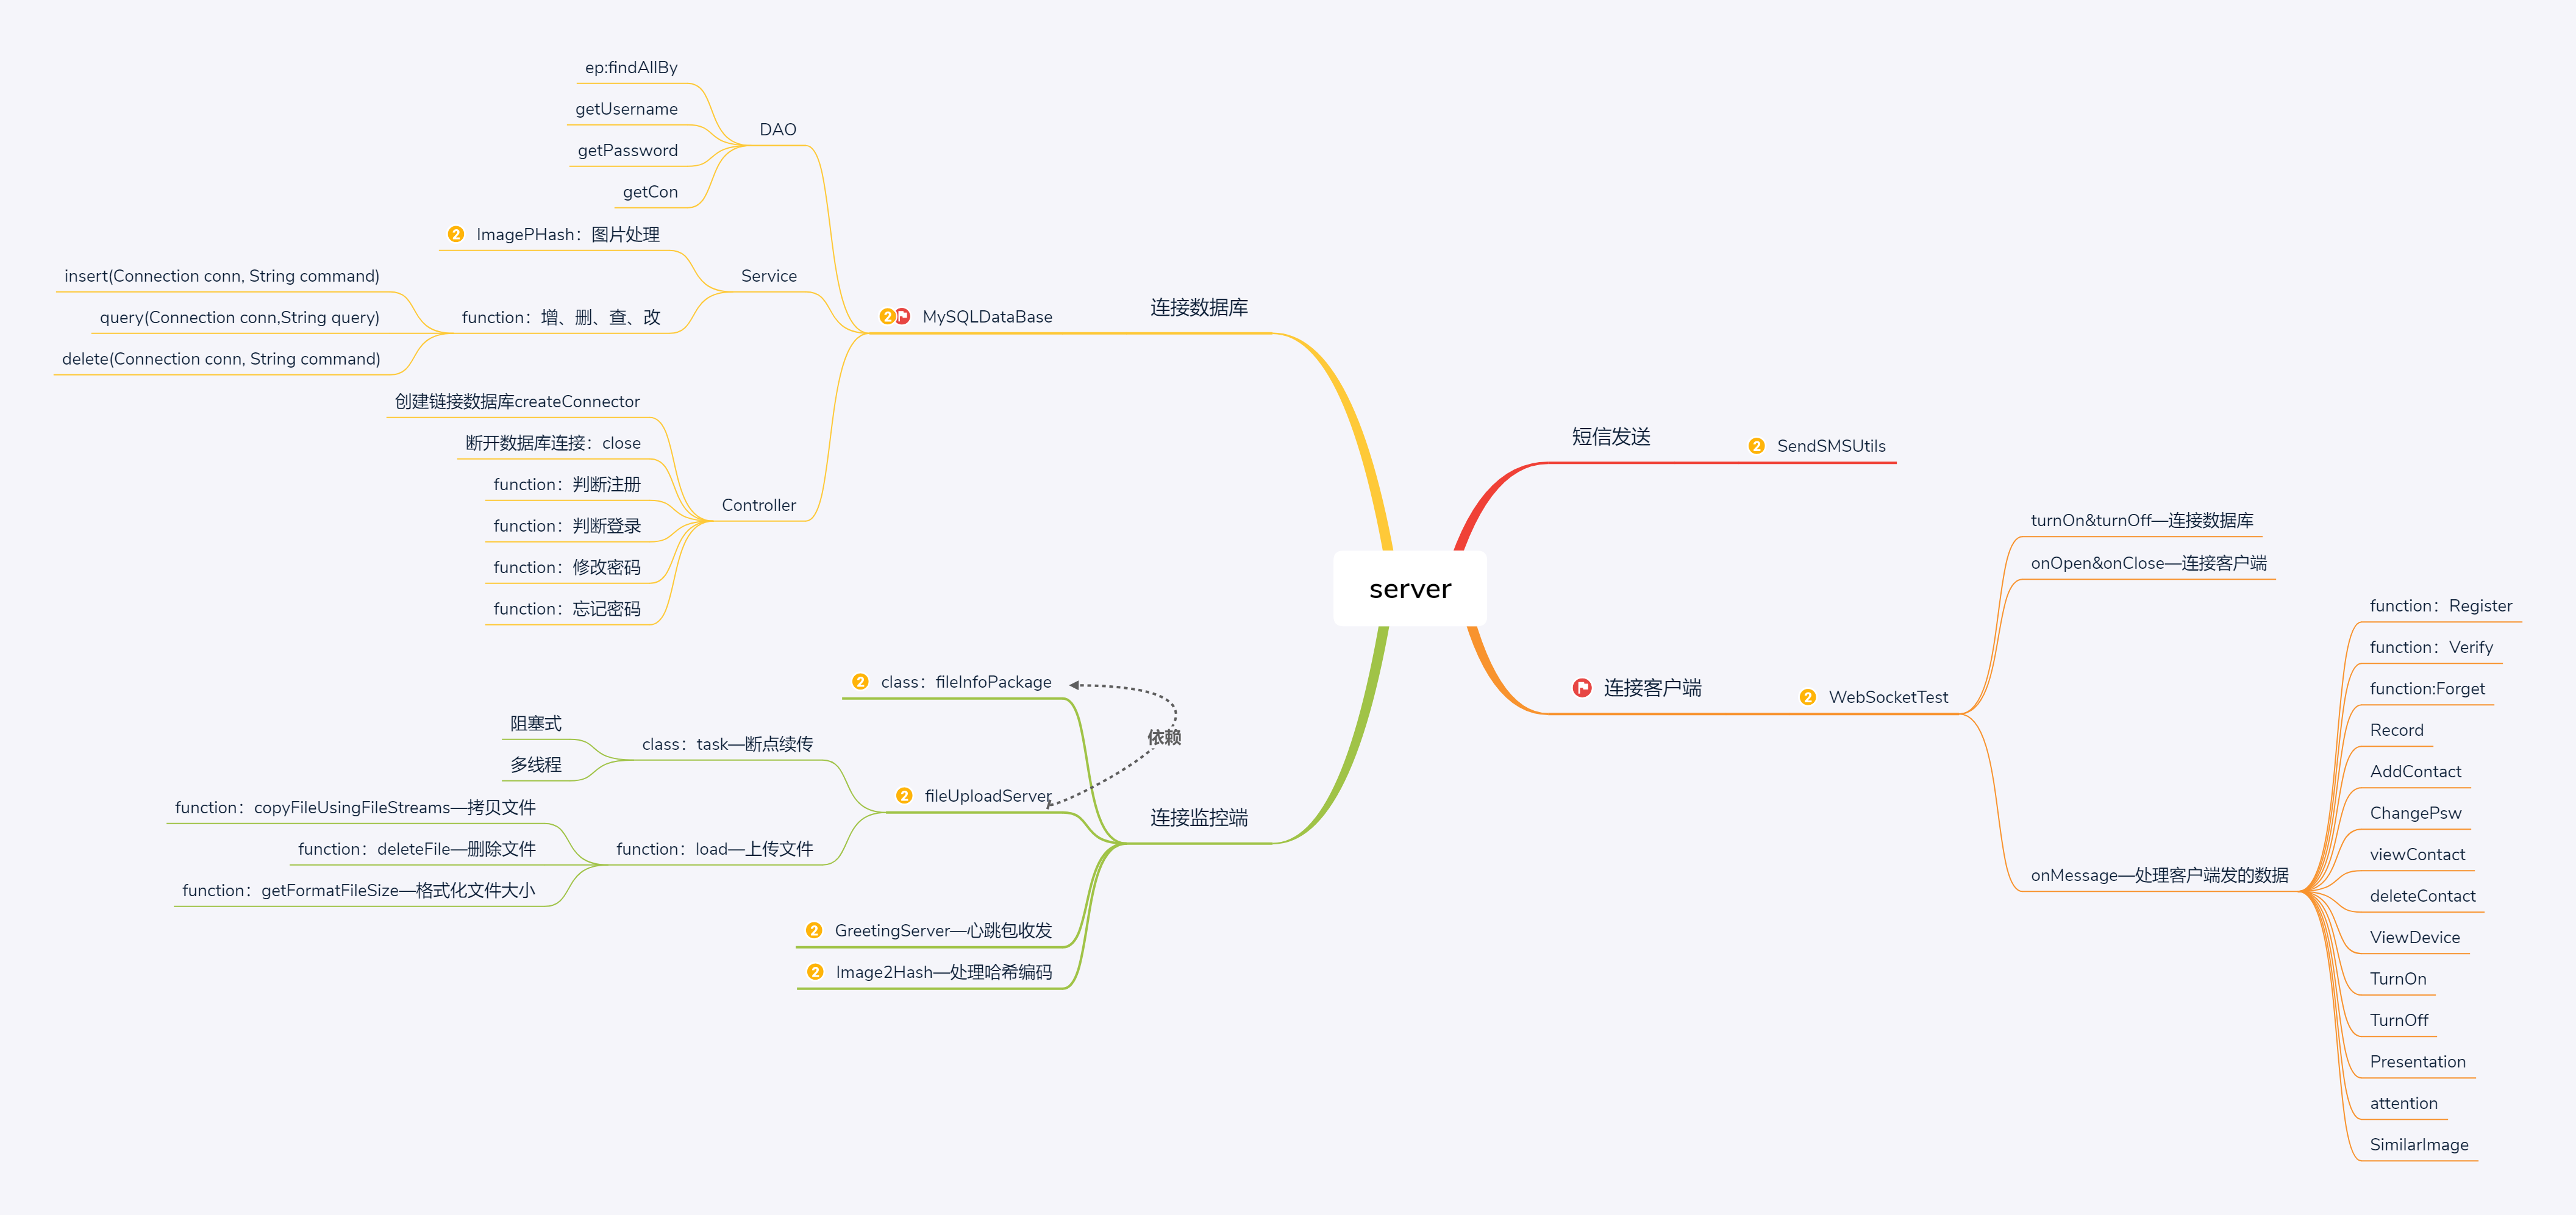
\includegraphics[scale=0.12]{img/5.png}
	\caption{服务器整体代码结构图}\label{fig:fig5}
\end{figure}

其中,连接监控端的代码结构如\textbf{图\ref{fig:fig6}}:

\begin{figure}[!htbp]
	\centering
	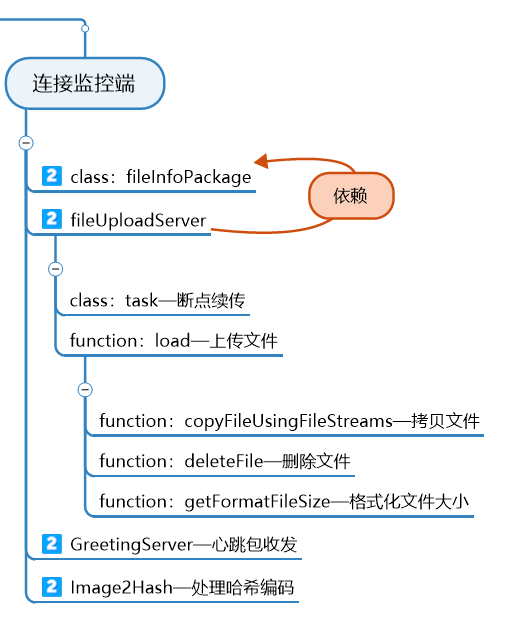
\includegraphics[scale=0.7]{img/6.png}
	\caption{服务器部分代码结构图}\label{fig:fig6}
\end{figure}

文件上传至服务器的类fileUploadServer与存储文件信息的类文件FileInfoPackage存在依赖关系,共同构成文件传输包FileUpload,结构如\textbf{图\ref{fig:fig7}}:

\begin{figure}[!htbp]
	\centering
	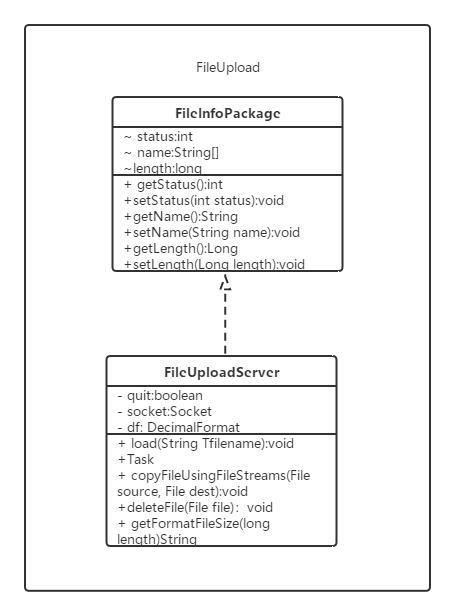
\includegraphics[scale=0.6]{img/7.png}
	\caption{服务器部分类图}\label{fig:fig7}
\end{figure}

fileUploadServer调用FileInfoPackage类部分代码:

\lstinputlisting[language=Java,firstline=1,lastline=10]{code/1.java}

\textbf{代码解析:}在fileUploadServer类中调用FileInfoPackage类,创建FileInfoPackage对象并进行数据包的属性(Status、Name、Length)设置,之后将FileInfoPackage的对象转换成json对象进行传输。

\textbf{原则分析:}此包满足高内聚性的原则,且具有单一的职责,即上传文件至服务器。包内的类FileInfoPackage只被fileUploadServer类所依赖,共同构成文件上传包FileUpload。FileUpload是可重用的,并且若要重用此包使其实现文件上传至服务器的功能,则必须重用包中所有的类。


\textbf{案例2:修正案例} 项目中客户端组件的代码结构如\textbf{图\ref{fig:fig8}}所示。各组件均在一个包中导致包的粒度较大,包的职责混乱。

\begin{figure}[!htbp]
	\centering
	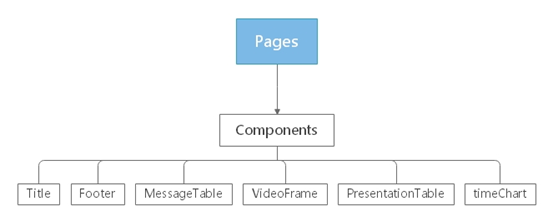
\includegraphics[scale=0.8]{img/8.png}
	\caption{客户端组件结构图}\label{fig:fig8}
\end{figure}

组件彼此间不存在依赖关系,重用某一个组件时,不会重用到其他组件,包的内聚性较差。

修改后的包结构如\textbf{图\ref{fig:fig9}}所示:

\begin{figure}[!htbp]
	\centering
	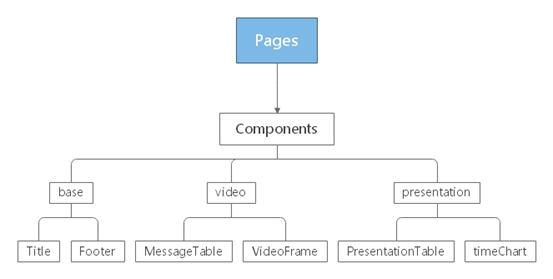
\includegraphics[scale=0.8]{img/9.png}
	\caption{客户端组件结构图(修改后)}\label{fig:fig9}
\end{figure}

修改后,业务逻辑分离得更彻底并保持完整。原组件包按功能分成了三个子包,分别是base包、video包和presentation包。包内的类彼此依赖,重用此包时需重用包中所有的类,具有高内聚性的特点。包的粒度由大粒度拆分为小粒度,分割了职责,减少包在重用的过程中的冗余。修改过后的项目,满足包的共同重用性(CRP)。

\subsubsection{共同封闭原则(CCP)}

\textbf{概念} 一个包中所有的类应该对同一种类型的变化关闭。一个变化影响一个包,便影响了包中所有的类。

\textbf{案例1} 原本的客户端组件都在同一个包中,如\textbf{图\ref{fig:fig16}}所示,违反共同封闭原则。

\begin{figure}[!htbp]
	\centering
	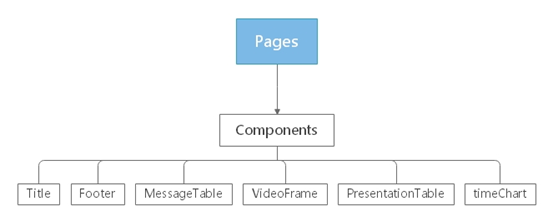
\includegraphics[scale=0.8]{img/8.png}
	\caption{客户端组件结构图}\label{fig:fig16}
\end{figure}

包中组件包括:
\begin{itemize}
	\item Title组件:页面的页眉菜单部分;
	\item Footer:页面的页脚部分;
	\item MessageTable:监控端有入侵后的文字信息显示,并以不同颜色标示出不同的危险等级;
	\item VideoFrame:监控端捕捉到的视频流实时展示;
	\item presentationTable:上月的入侵监控报告文字说明;
	\item timeChart:上月入侵监控报告汇总柱状图;
\end{itemize}

修改后包结构如\textbf{图\ref{fig:fig17}}显示:

\begin{figure}[!htbp]
	\centering
	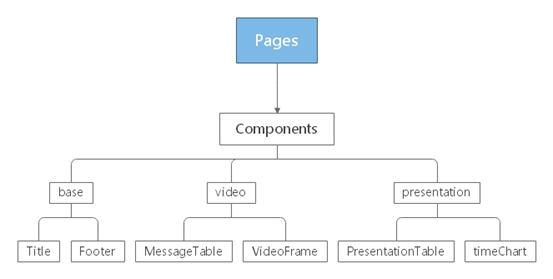
\includegraphics[scale=0.8]{img/9.png}
	\caption{客户端组件结构图(修改后)}\label{fig:fig17}
\end{figure}
\newpage
修改后将footer、title两个页面基础组件放入同一个包中,面对页面基础结构需求封闭;MessageTable和VideoFrame两个组件放入同一个包中,面对实时入侵监控需求封闭;presentationTable和timeChart两个组件放入同一个包中,面对入侵情况汇总需求封闭,实现共同封闭原则。

\textbf{案例2} 原本的服务器端没有分包,违反共同封闭原则。

原服务器各类协作完成与客户端、监控器端的交互,其中Image2Hash类和ImageHash类主要负责图片处理,FileUploadServer、FileInfoPackage、GreetingsServer主要负责服务器与监控端的交互,WebSocketTest主要负责服务器与客户端的交互,SendSMSUtils负责短信发送。

原服务器文件结构如\textbf{图\ref{fig:fig18}}:

\begin{figure}[!htbp]
	\centering
	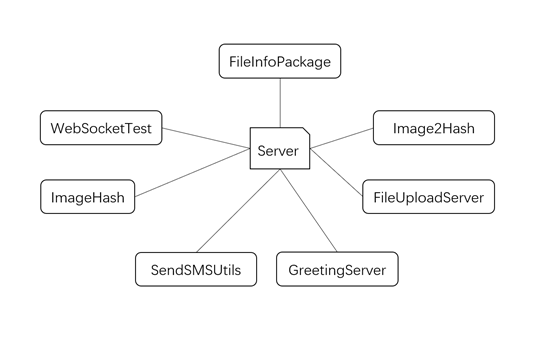
\includegraphics[scale=0.5]{img/15.png}
	\caption{服务器文件结构图}\label{fig:fig18}
\end{figure}

修改后服务器文件结构如\textbf{图\ref{fig:fig19}}:

\begin{figure}[!htbp]
	\centering
	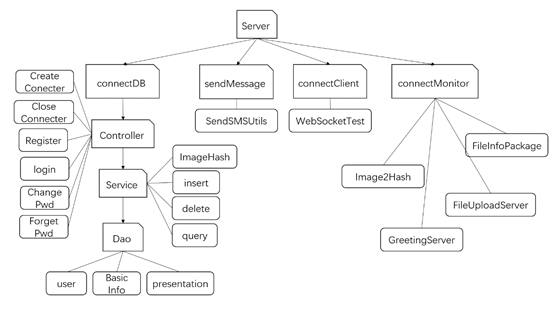
\includegraphics[scale=0.8]{img/16.png}
	\caption{服务器文件结构图(修改后)}\label{fig:fig19}
\end{figure}

将FileUploadServer、FileInfoPackage、GreetingsServer、Image2Hash放入同一个包中,面对连接监控端需求封闭;将WebSocketTest放入一个包内,面对连接客户端需求封闭;将SendSMSUtils放入一个包内,面对发送短信需求封闭;将原本连接数据库的代码更改为springboot架构,拆分为dao、service、controller三个包,controller包依赖service包,service包依赖dao包,他们共同放在connectDB包中,面对连接数据库的需求封闭。实现共同封闭原则。


\subsubsection{无环依赖原则(ADP)}
\textbf{概念} 在包依赖关系图中不允许环的存在。

\textbf{案例} 原项目中客户端的依赖关系是客户端依赖于页面,页面依赖于组件,该结构不存在环,符合无环依赖原则。首先完成title、footer等基础组件的开发,再完成pages中的页面开发,可以完成自底向上的增量式开发,解决早后综合征的问题。

原项目中服务器端原本没有依赖关系,修改后服务器端依赖于connectDB、sendMessage、connectClient、connectMonitor四个包,connectDB包依赖于controller包,controller包依赖于service包,service包依赖于dao包,该结构不存在环,符合无环依赖原则。开发时先完成dao包的开发,再依次完成service包、controller包的开发,最后完成connectDB、sendMessage、connectClient、connectMonitor四个包的开发,实现自底向上的增量式开发。

\subsubsection{稳定依赖原则(SDP)}
\textbf{概念} 顺着稳定的方向依赖,该原则可以确保不稳定的模块依赖稳定的模块。

\textbf{案例1} 在我们所选择的项目中前端的包管理中使用到了稳定依赖原则。

pages包:页面的展示包,主要是一些功能模块比如注册登录,展示信息等。
Components包:页面的组件包,主要是用于页面展示功能组件。
在未修改其符合共同封闭原则前的包依赖关系如\textbf{图\ref{fig:fig20}}:

\begin{figure}[!htbp]
	\centering
	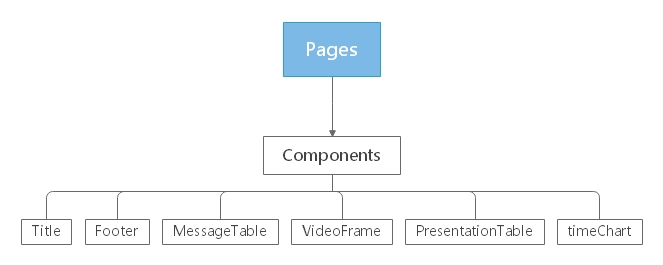
\includegraphics[scale=0.8]{img/17.jpg}
	\caption{前端分包示意图}\label{fig:fig20}
\end{figure}

可以看到pages包依赖于components组件包,这里项目设计就是pages包去调用组件包中的组件来构建页面。明显pages包的I值大于它所依赖的components包的I值

在修改其符合共同封闭原则后的包依赖关系如\textbf{图\ref{fig:fig21}}:
\begin{figure}[!htbp]
	\centering
	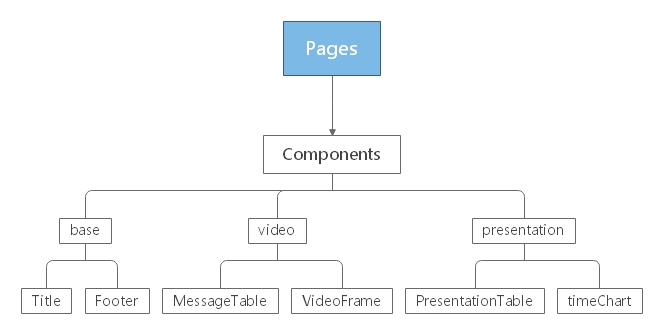
\includegraphics[scale=0.8]{img/18.jpg}
	\caption{前端分包示意图(修改后)}\label{fig:fig21}
\end{figure}

可以看到修改完后仍然是符合稳定依赖原则。

\textbf{案例2} 后端的包管理中修改之前是没有包管理的,server端我们将所有的文件全部放一个包下了,这是不符合包管理的原则的。修改完之后
	在之前的图的基础上,我们重点分析\textbf{图\ref{fig:fig22}}的这部分:
	
	\begin{figure}[!htbp]
		\centering
		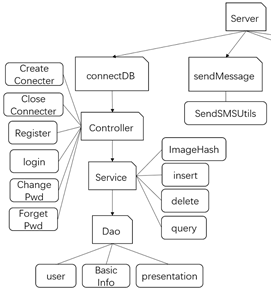
\includegraphics[scale=1.5]{img/21.png}
		\caption{服务器分包示意图(修改后)}\label{fig:fig22}
	\end{figure}
	
	可以看到从connectDB依赖于controller,controller依赖于service,service依赖于dao层。I值从上往下递减,越往下越稳定。符合稳定依赖原则。
	
\subsubsection{稳定抽象原则(SAP)}

\textbf{概念} 稳定的包应该是抽象的,其稳定性不应该妨碍它被扩展。

\textbf{案例1} 接前一个稳定依赖原则的前端包关系,我们发现这里并没有遵循稳定抽象原则。因为组件包应该要是一个稳定的包,但是我们有时候也需要去修改包里面的文件,比如修改页眉、页脚,以及修改功能组件。而采用原先的架构他并不抽象,不好扩展。于是我们运用稳定抽象原则,设计一个接口层,让base、video、presentation里的文件去实现这个接口。修改后的架构如\textbf{图\ref{fig:fig23}}:

\begin{figure}[!htbp]
	\centering
	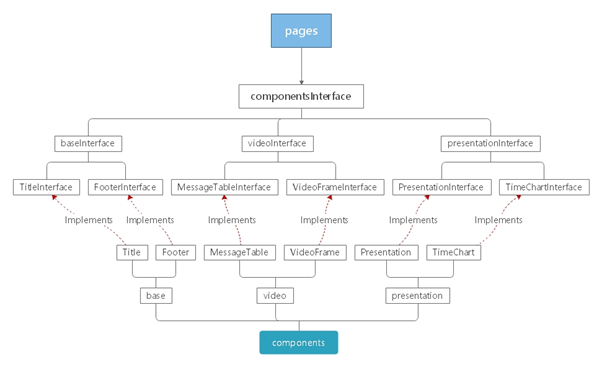
\includegraphics[scale=0.8]{img/14.png}
	\caption{前端包示意图(修改后)}\label{fig:fig23}
\end{figure}

\newpage

\textbf{案例2} 后端的包结构关系中也没有遵循稳定抽象原则,service依赖的dao层是稳定的但是也需要是抽象的,因为我们有可能更换数据库管理软件,比如从mysql换成oracle,这里我们设计一个数据库持久层充当接口层,修改后的这部分架构如\textbf{图\ref{fig:fig24}}:

\begin{figure}[!htbp]
	\centering
	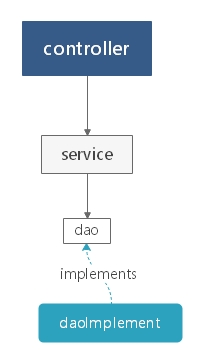
\includegraphics[scale=0.8]{img/20.jpg}
	\caption{数据库分包示意图(修改后)}\label{fig:fig24}
\end{figure}
\end{document}